\documentclass[12pt, letterpaper]{report}
\usepackage{graphicx}
\usepackage{hyperref}
\usepackage{amssymb}
\usepackage{amsmath}
\usepackage{float}
\usepackage{mathtools}
\usepackage{enumitem}
\usepackage[margin=1in]{geometry}
\usepackage[figurename=Figura]{caption}
\title{Tarea 1. Análisis Estadístico}
\author{Juan Pablo Guerrero Escudero, A01706810}
\date{20 mayo, 2024}
\begin{document}
\maketitle
\begin{enumerate}
\item \textbf{Ejercicio 1}: 
Datos: $M = 5000 hrs$, $\sigma = 100 hrs$. $X \sim N(5000, 100^2)$. Para encontrar $P(x \leq 4500)$, estandarizamos 
el problema de manera $Z = \frac{x - M}{\sigma}$. En éste caso, $Z = \frac{X - 5000}{100}$ y si queremos encontrar $x = 4500$, 
sustituimos en lo anterior, lo que resulta en $P(Z \leq \frac{4500 - 5000}{100}) = P(Z \leq -5)$. Al ingresar éste valor en 
la calculadora de la distribución normal, $P(x \leq -5) = 0$. Podemos comprobarlo al ilustrar la gráfica de la región de la 
distribución: 
\begin{figure}[H]
    \centering
    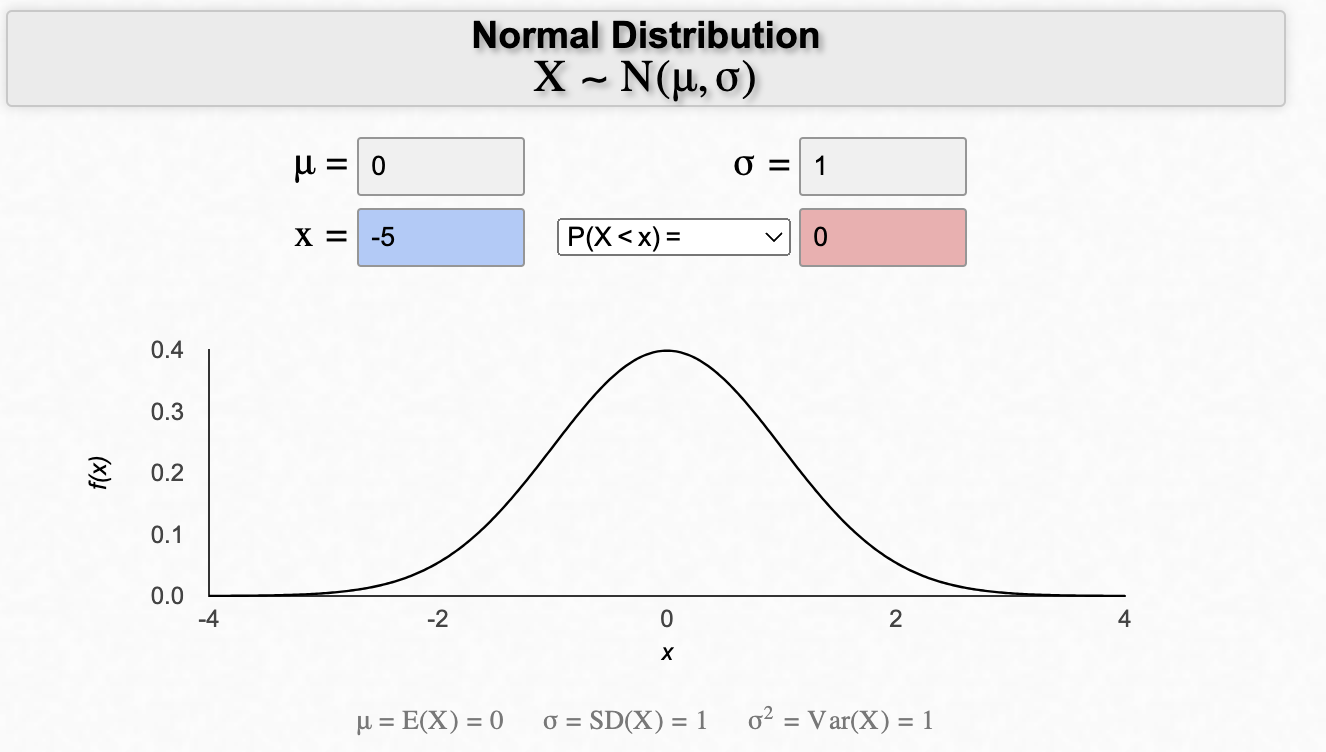
\includegraphics[height = 7cm]{Fig1_DistribucionNormal_P1T1_AnalisisEstadistico.png}
    \caption{Diagrama de gráfica problema 1}
\end{figure}
Éste valor se encuentra muy alejada en la parte de la izquierda de la curva y es muy cercana a cero. 
\item \textbf{Ejercicio 2}: ¿Cuáles de las siguientes afirmaciones describe correctamente el significado
de un intervalo de confianza del 95 por ciento?     
\begin{enumerate}
\item Ésto es correcto ya que la definición de un intervalo de confianza nos dice que de 100 intervalos obtenidos 
de la msma manera, aproximadamente $\beta $ de ellos contendrán a la media verdadera $M$. En éste caso, la media 
poblacional efectivamente se encontrará en aproximadamente el $95$\% de esos intervalos con ese porcentaje de 
nivel de confianza. 
\item Ésto es incorrecto ya que lo que un intervalo de confianza nos dice es qué porcentaje de los intervalos 
creados contienen a la media verdadera o media poblacional, no la media muestral. Es decir, un intervalo de confianza del $95$\% 
significa que estamos 95\% seguros que el intervalo calculado contiene a la media poblacional. 
\item Ésto es incorrecto ya que un intervalo de confianza no nos asegura un porcentaje de datos de la población que se encuentren 
dentro de ése intervalo. Para calcular ésto, se usan teoremas como el de Chevychev para calcular el porcentaje de datos dentro de 
un intervalo que parte de la media + $n$ desviaciones estándar. 
\item Ésto es incorrecto ya que solo existe una media poblacional. Un intervalo de confianza dice que al tomar muestras y calcular sus 
medias, aproximadamente $95$\% de ésos intervalos contendrán a la verdadera media poblacional. No existen múltiples 
medias poblacionales, solo múltiples medias muestrales. 
\end{enumerate}
\item \textbf{Ejercicio 3}: 
\begin{enumerate}
\item Intervalo de confianza de $95$\% con $n = 25$ motores y carga parásita promedio de $58.3$. \\
Datos: $\alpha = 0.05$, $n = 25$, $\bar{x} = 58.3$. Cálculo de intervalo: 
\begin{align*}
    IC &= (58.3 - Z_{0.0025}(\frac{3}{\sqrt{25}}), 58.3 +  Z_{0.0025}(\frac{3}{\sqrt{25}}))\\ 
    IC &= (58.3 - 1.95996(\frac{3}{\sqrt{25}}), 58.3 +  1.95996(\frac{3}{\sqrt{25}}))\\
    IC &= (57.1240, 59.47598)
\end{align*}
\item Intervalo de confianza de $95$\% con $n = 100$ motores y carga parásita promedio de $58.3$. \\
Datos: $\alpha = 0.05$, $n = 100$, $\bar{x} = 58.3$. Cálculo de intervalo: 
\begin{align*}
    IC &= (58.3 - Z_{0.0025}(\frac{3}{\sqrt{100}}), 58.3 +  Z_{0.0025}(\frac{3}{\sqrt{100}}))\\ 
    IC &= (58.3 - 1.95996(\frac{3}{\sqrt{100}}), 58.3 +  1.95996(\frac{3}{\sqrt{100}}))\\
    IC &= (57.7120, 58.88799)
\end{align*}
\item Intervalo de confianza de $99$\% con $n = 100$ motores y carga parásita promedio de $58.3$. \\
Datos: $\alpha = 0.01$, $n = 100$, $\bar{x} = 58.3$. Cálculo de intervalo: 
\begin{align*}
    IC &= (58.3 - Z_{0.0005}(\frac{3}{\sqrt{100}}), 58.3 +  Z_{0.0005}(\frac{3}{\sqrt{100}}))\\ 
    IC &= (58.3 - 2.5758(\frac{3}{\sqrt{100}}), 58.3 +  2.5758(\frac{3}{\sqrt{100}}))\\
    IC &= (57.52726, 59.07274)
\end{align*}
\item Intervalo de confianza de $82$\% con $n = 100$ motores y carga parásita promedio de $58.3$. \\
Datos: $\alpha = 0.18$, $n = 100$, $\bar{x} = 58.3$. Cálculo de intervalo: 
\begin{align*}
    IC &= (58.3 - Z_{0.09}(\frac{3}{\sqrt{100}}), 58.3 +  Z_{0.09}(\frac{3}{\sqrt{100}}))\\ 
    IC &= (58.3 - 1.34076(\frac{3}{\sqrt{100}}), 58.3 +  1.34076(\frac{3}{\sqrt{100}}))\\
    IC &= (57.8978, 58.7022)
\end{align*}
\item Compare las respuestas de los items anteriores y argumente sus diferencias: \\ 
\textbf{Respuesta: } Observando los intervalos obtenidos, se aprecia que el intervalo para $n = 25$ es más grande que todos los 
demás, lo que es correcto ya que mientras más grande sea la muestra, más se acerca $\bar{x}$ a una distribución normal debido a que 
mientras la muestra aumenta, más se reduce la amplitud del intervalo de confianza. En éste caso, como se tiene una muestra más pequeña, 
se espera un intervalo más grande que para muestras más grandes en cantidad. Después, en los siguientes 
tres intervalos se observa que mientras más se reduce el porcentaje de confianza, más se reduce el intervalo, siendo el intervalo de confianza 
para $82$\% el más chico de los tres. 
\item ¿Qué tan grande debe ser la muestra si el ancho del intervalo debe ser de 1.0?
Asumiendo que estamos buscando una distribución normal, y buscamos un nivel de confianza del $96$\%, entonces 
la fórmula para el tamaño de intervalo es $2(Z_{\frac{\alpha}{2}}\ast \frac{\mu}{\sqrt{n}})$. Podemos igualar ésta expresión a 1 y resolver para n para 
encontrar el tamaño de muestra necesario. 
\begin{align*}
    1 &= 2(Z_{\frac{0.05}{2}}\ast \frac{3}{\sqrt{n}})\\
    1 &= 2(1.95996(\frac{3}{\sqrt{n}}))\\
    \frac{1}{3.91992} &= \frac{3}{\sqrt{n}}\\
    \sqrt{n} &= 11.79976\\
    n &= 138.29196
\end{align*}
Por lo que para que el tamaño de intervalo sea de 1, necesitamos aproximadamente una muestra de $138$ elementos después de redondear. 
\end{enumerate}
\item \textbf{Ejercicio 4}: Calcular intervalo de confianza de $99$\% para $\mu$ e interpretar. \\ 
Datos: $n = 110$, $\bar{x} = 0.81$, $S = 0.34$, $\alpha = 0.01$. 
\begin{align*}
IC &= (0.81 - t_{\frac{0.01}{2}, 110 - 1} \ast \frac{0.34}{\sqrt{110}}, 0.81 + t_{\frac{0.01}{2}, 110 - 1} \ast \frac{0.34}{\sqrt{110}})\\
IC &= (0.81 - 2.67995 \ast \frac{0.34}{\sqrt{110}}, 0.81 +  2.67995 \ast \frac{0.34}{\sqrt{110}})\\ 
IC &= (0.7231, 0.8969)
\end{align*}
El intervalo de confianza de $99$\% para la media poblacional $\mu$ es $(0.7231, 0.8969)$, es decir de 100 
muestras aleatorias, la media se encontrará dentro del 95\% de esos intervalos. El intervalo es relativamente grande ya que 
el intervalo de confianza que se busca es mayor, y por lo tanto se necesita un rango más amplio para asegurarse de que la media 
se encuentre dentro de ése intervalo el 99\% de las veces. 
\item \textbf{Ejercicio 5}: Se utiliza la fórmula para el Caso 3 del cálculo de intervalos de confianza, debido a que 
tenemos una muestra a la cuál podemos obtener su media y desviación muestral, y encontrar $\mu$ o la media poblacional. Cálculo de 
intervalo. De datos obtenidos tenemos $\bar{x} = 10$, $S_x = 0.08$, $\alpha = 0.05$, $n = 7$. 
\begin{align*}
IC &= (\bar{x} - t_{\frac{\alpha}{2}, n-1}(\frac{S}{\sqrt{n}}), \bar{x} + T_{\frac{0.05}{2}, 6}(\frac{0.08}{\sqrt{7}}) )\\
IC &= (10- T_{\frac{0.05}{2}, 6}(\frac{0.08}{\sqrt{7}}), 10 +T_{\frac{0.05}{2}, 6}(\frac{0.08}{\sqrt{7}}))\\
IC &= (10-(2.4469)(\frac{0.08}{\sqrt{7}}), 10 + (2.4469)(\frac{0.08}{\sqrt{7}}))\\ 
IC &= (9.9260, 10.07399)
\end{align*}
Y por lo tanto, asumiendo que la población se comporta como una distribución normal, de 100 intervalos generados, el 95\% de 
las veces la media poblacional para el contenido medio de todos los contenedores se encontrará en el intervalo 
calculado. 
\item \textbf{Ejercicio 6}: Para éste ejercicio, para el cálculo del intervalo de confianza se usa la fórmula para el 
Caso 2 debido a que tenemos una muestra grande $(n > 30)$, podemos calcular la desviación muestral, y la desviación poblacional es desconocida. 
En éste caso, la fórmula y cálculos se muestran a continuación. En éste caso la media muestral $\bar{x} = 54.6735, S = 26.8495$, $n = 49$, $\alpha = 0.05$: 
\begin{align*}
IC &= (\bar{x} - Z_{\frac{\alpha}{2}}(\frac{S}{\sqrt{n}}), \bar{x} + Z_{\frac{\alpha}{2}}(\frac{S}{\sqrt{n}}))\\ 
IC &= (54.6735 - Z_{\frac{0.05}{2}}(\frac{26.8495}{\sqrt{49}}), 54.6735 + Z_{\frac{0.05}{2}}(\frac{26.8495}{\sqrt{49}}))\\
IC &= (54.6735 - (1.95996)(\frac{26.8495}{\sqrt{49}}), 54.7635 + (1.95996)(\frac{26.8495}{\sqrt{49}}))\\ 
IC &= (47.15579, 67.19121)
\end{align*}
En éste caso, el cálculo del intervalo de confianza para el promedio real de voltaje de ruptura $\mu$ es bastante amplio, lo cuál 
nos indica que no hay mucha precisión en la estimación de $\mu$. Ésto se debe a varias razones. en primer lugar, existe una variabilidad considerable 
dentro de la muestra de los datos, con una desviación muestral de magnitud relativamente considerable. En segundo lugar, el tamaño de la muestra 
no es lo suficientemente grande como para disminuir el error que viene de parte de la desviación muestra. Para ser más precisos, se podría 
aumentar el tamaño de la muestra o reducir la variabilidad de los datos. 
\end{enumerate}
\end{document}